\documentclass{beamer}
\mode<presentation>
{\usetheme{Rochester}}
\usepackage[orientation=portrait,size=a1,scale=0.9]{beamerposter}

%% %%%%%%%%%%%%%%%%%%%%%%%%%%%%%%%%%%%%%%%%%%%%%%%%%%%%%%%%%%%%%%%%%%%%%%%%%%%%%
%% %%%%%%% %% %% %  %                                      %  % %% %% %%%%%%%%%%
%%%%% %% %  %                    MES COMMANDES                     %  % %% %%%%%
%%%%%%%%%% %% %% %  %                                      %  % %% %% %%%%%%% %%
%%%%%%%%%%%%%%%%%%%%%%%%%%%%%%%%%%%%%%%%%%%%%%%%%%%%%%%%%%%%%%%%%%%%%%%%%%%%% %%


\def\zzpackages{
  \usepackage[utf8]{inputenc}
  \usepackage[T1]{fontenc}
%  \usepackage[french]{babel}

  \usepackage{amsthm}
  \usepackage{amsmath}
  \usepackage{amsfonts}
  \usepackage{amssymb}

  \usepackage{xcolor}
  \usepackage{xstring}	%\ifstreqcase
}

%% %%%%%%%%%%%%%%%%%%%%%%%%%%%%%%%%%%%%%%%%%%%%%%%%%%%%%%%%%%%%%%%%%%%%%%%%%%%%%
%                              TESTS / FOR / ...                               %
%%%%%%%%%%%%%%%%%%%%%%%%%%%%%%%%%%%%%%%%%%%%%%%%%%%%%%%%%%%%%%%%%%%%%%%%%%%%% %%

% 
\def\defactive#1#2{
  \catcode`#1=13
  \begingroup
  \lcode`~=`#1
  \lowercase{\endgroup\def~}{#2}
}

\def\zifempty#1#2#3{\def\foo{#1}\ifx\foo\empty\relax#2\else#3\fi}

%% %%%%%%%%%%%%%%%%%%%%%%%%%%%%%%%%%%%%%%%%%%%%%%%%%%%%%%%%%%%%%%%%%%%%%%%%%%%%%
%                           MARGES / HYPERREF / ...                            %
%%%%%%%%%%%%%%%%%%%%%%%%%%%%%%%%%%%%%%%%%%%%%%%%%%%%%%%%%%%%%%%%%%%%%%%%%%%%% %%

\makeatletter
\gdef\@subtitle{}
\def\subtitle#1{\gdef\@subtitle{#1}}

\def\zztitre{
\begingroup\centering
{\bfseries \huge \@title}\par\vspace{.3cm}
\ifx\@subtitle\empty\else{\bfseries \Large \@subtitle}\par\vspace{.5cm}\fi
\Large \@author\par\vspace{.1cm}
\@date\zal\vspace{.3cm}\zal
\zligne\endgroup
}

\makeatother


\newcommand{\zzhyperref}{
\usepackage{hyperref}
\hypersetup{ colorlinks=true, linkcolor=blue!30!black,
citecolor=green!30!black, filecolor=magenta!30!black,
urlcolor=cyan!30!black }
}

\newcommand{\zzmarges}{
  \setlength{\textheight}{620pt}
  \addtolength{\textwidth}{2cm}
  \addtolength{\hoffset}{-1cm}
  \addtolength{\voffset}{-1cm}
  \addtolength{\marginparwidth}{0cm}
  \addtolength{\textheight}{1cm}
} 

\makeatletter
\newcommand{\zzheader}[6]{
\def\@oddhead{\vbox to 0pt{\vss\hspace{0pt} #1\hfill #2\hfill #3\kern4pt\par\kern5pt\hrule height.5pt}}
\def\@oddfoot{\vbox to 0pt{\hrule height.5pt\kern5pt\hbox to \linewidth{\kern4pt {#4}\hss {#5}\hss {#6}\kern4pt}\vss}}}
\makeatother

%%%%%%%%%%%%%%%%%%%%%%%%%%%%%%%%%%%%%%%%%%%%%%%%%%%%%%%%%%%%%%%%%%%%%%%%%%%%%%%%

\newcommand{\zligne}[1][]{
\par\zifempty{#1}%
{\hbox to \linewidth{\leaders\hrule height3pt depth-2.5pt\hfill}}%
{\hbox to \linewidth{\leaders\hrule height3pt depth-2.5pt\hfill\kern.8em #1\kern.8em\leaders\hrule height3pt depth-2.5pt\hfill}}\par
}

%%%%%%%%%%%%%%%%%%%%%%%%%%%%%%%%%%%%%%%%%%%%%%%%%%%%%%%%%%%%%%%%%%%%%%%%%%%%%%%%

\newcommand{\zal}{\par}
\newcommand{\znl}{\zal ~\zal}
\newcommand{\zguill}[2][]{«\,#2\,»}

%% %%%%%%%%%%%%%%%%%%%%%%%%%%%%%%%%%%%%%%%%%%%%%%%%%%%%%%%%%%%%%%%%%%%%%%%%%%%%%
%                             COMMANDES PRATIQUES                              %
%%%%%%%%%%%%%%%%%%%%%%%%%%%%%%%%%%%%%%%%%%%%%%%%%%%%%%%%%%%%%%%%%%%%%%%%%%%%% %%

%% ------- -- -- -  -                                      -  - -- -- --------%%
%---- -- -  -                          ZP                          -  - -- ----%
%%-------- -- -- -  -                                      -  - -- -- ------- %%
\makeatletter
\def\z@first#1#2{#1}
\def\z@second#1#2{#2}
\def\z@zp@selectchar#1#2{
  \IfStrEqCase{#2}{%
    {p}{#1{(}{)}}%
    {c}{#1{[}{]}}%
    {a}{#1{\{}{\}}}%
    {C}{#1{]}{[}}%
    {b}{#1{|}{|}}%
    {n}{#1{\|}{\|}}%
    {i}{#1{[}{]}\!#1{[}{]}}%
    {t}{#1{<}{>}}%
    {v}{#1{.}{.}}%
    {A}{#1{\}}{\{}}%
    {P}{#1{)}{(}}%
    {I}{#1{]}{[}\!#1{]}{[}}%
    {T}{#1{>}{<}}%
  }[#1{(}{)}]%
}

\def\z@zp#1#2\fin#3{
  \z@zp@selectchar{\left\z@first}{#1}#3
  \zifempty{#2}%
        {\z@zp@selectchar{\right\z@second}{#1}}%
        {\z@zp@selectchar{\right\z@second}{#2}}%
}
\newcommand{\zp}[2][]{\zifempty{#1}{\left(#2\right)}{\z@zp#1\fin{#2}}}

\newcommand{\zpbig}[1]{\ifcase#1\relax\vrule width0pt height0pt\or\vrule width0pt height9pt\or\vrule width0pt height10pt\or\vrule width0pt height13pt\else\vrule width0pt height16pt\fi}

%% ------- -- -- -  -                                      -  - -- -- --------%%
%---- -- -  -                        AUTRES                        -  - -- ----%
%%-------- -- -- -  -                                      -  - -- -- ------- %%


\newcommand{\zsum}[2][0pt]{\sum_{\hbox to #1{\hss$\scriptstyle#2$\hss}}}
\newcommand{\zprod}[2][0pt]{\prod_{\hbox to #1{\hss$\scriptstyle#2$\hss}}}

\newcommand{\zseq}[1][=]{\hspace{2pt}\raise .5pt\hbox{\scalebox{.8}{#1}}\hspace{2pt}}

\newcommand{\zop}[2]{\mathrm{#1}\zp{#2}}

\newcommand{\zi}{\mathrm{i}}

\newcommand{\zexp}[1]{\mathrm{e}^{#1}}

\newcommand{\zmatrix}[2]{\left(\begin{array}{#1}#2\end{array}\right)}

\newcommand{\zindic}[1]{%
\hbox to 5.3pt{1\hss l}\hskip -2.5pt\left\{#1\right\}%
}

\newcommand{\zesp}[2][]{%              esperance
\mathbb{E}_{#1}\hskip -3pt\left[\zpbig1\,#2\,\right]%
}

\newcommand{\zprob}[2][]{%             proba
\mathbb{P}_{#1}\hskip -3pt\left(\zpbig1\,#2\,\right)%
}

% Symbole d'indépendance de variable aléatoire
\newcommand{\zindep}{\protect\mathpalette{\protect\z@ind}{\perp}}
\def\z@ind#1#2{\mathrel{\rlap{$#1#2$}\mkern6mu{#1#2}}}


\newcommand{\zdx}[1]{\mathrm{d}#1}

\newcommand{\zderiv}[2]{\frac{\partial #1}{\partial #2}}


\newcommand{\ztr}[2][]{\zifempty{#1}{#2}{\left(#2\right)}^{\hspace{-1pt}\mathsf{T}}\hspace{-1pt}}
\def\zpreind#1#2{ \raise-.35ex\hbox{\scriptsize$#1$}#2}
\def\zpreexp#1#2{ \raise.85ex\hbox{\scriptsize$#1$}#2}

%% %%%%%%%%%%%%%%%%%%%%%%%%%%%%%%%%%%%%%%%%%%%%%%%%%%%%%%%%%%%%%%%%%%%%%%%%%%%%%
%                                 ALGORITHMES                                  %
%%%%%%%%%%%%%%%%%%%%%%%%%%%%%%%%%%%%%%%%%%%%%%%%%%%%%%%%%%%%%%%%%%%%%%%%%%%%% %%

\newcount\z@algo@count
\newdimen\z@algo@indent
\begingroup
  \catcode`\^^M=13             %
  \catcode`\^^I=13             %
  \gdef\z@algo{                %
  \z@algo@count=1
    \begingroup                %
    \catcode`\^^M=13           %
    \def^^M{\leavevmode\par \advance\z@algo@count by 1\z@algo@indent=0pt}%
    \catcode`\^^I=13           %
    \def^^I{\advance\z@algo@indent by 1em}         %
    \everypar{                 %
      \hbox to 0cm{\hss\textcolor{black!30}{\the\z@algo@count~:}}~\kern\z@algo@indent}  %
                               %
    \tt                        %
  }

\endgroup

\newenvironment{zalgo}{\z@algo}{\endgroup}


\makeatother



%% %%%%%%%%%%%%%%%%%%%%%%%%%%%%%%%%%%%%%%%%%%%%%%%%%%%%%%%%%%%%%%%%%%%%%%%%%%%%%
%                                    AUTRE                                     %
%%%%%%%%%%%%%%%%%%%%%%%%%%%%%%%%%%%%%%%%%%%%%%%%%%%%%%%%%%%%%%%%%%%%%%%%%%%%% %%

% epaisseur trait / marge / texte

\def\zfbox#1#2#3{
  \hbox{\vrule width #1
    \vtop{
      \vbox{
        \hrule height #1
        \kern #2
        \hbox{\kern #2 #3\kern #2}
      }%
      \kern #2%
      \hrule height #1
    }%
    \vrule width #1%
  }%
}

%% \begin{mygraph}{xmin=0, xmax=1, %
%%                ymin=0, ymax=1, %
%%                sizex=2.5, sizey=2.5}%
%%                {nomx=Axe X, nomy=Axe Y}%
%%                {0,.5,1}{0,0.25,...,1.05}

%% \graduationX[dashed, blue]{ .78 / $\frac{\pi}{4}$ }{ PARAMETRE TEXT }

%% \begin{mylegend}{x=0.3, y=.9, n=2, t=2.1, scale=.5}
%%   \newlegend{blue}{Courbe 1}
%%   \newlegend{red}{Courbe 2}
%% \end{mylegend}

%% \fillbetweencurve[opacity=.2, blue]{ COURBE 1 }{ COURBE 2 }

%% \end{mygraph}


\usepackage{tikz}



\pgfkeys{
%
 /mygraph/.is family, /mygraph,
 xmin/.estore in = \xn,
 xmax/.estore in = \xm,
 ymin/.estore in = \yn,
 ymax/.estore in = \ym,
 sizex/.estore in = \xx,
 sizey/.estore in = \yy,
 %
/mygraphb/.is family, /mygraphb,
 nomx/.estore in = \axex,
 nomy/.estore in = \axey,
%
/mygraphc/.is family, /mygraphc,
 gradsize/.estore in = \gradsize,
 gradsize/.default = 0.1,
 nomydist/.estore in = \axeyd,
 nomydist/.default = 0.8cm,
 gradsize, nomydist,                 % NE PAS OUBLIER
%
/myleg/.is family, /myleg,
 x/.estore in = \legendx,
 y/.estore in = \legendy,
 n/.estore in = \legendn,
 t/.estore in = \legendt,
 scale/.estore in = \legends,
 scale/.default = 1,
 scale,
%
/mylego/.is family, /mylego,
size/.estore in = \legendwidth,
size/.default = 0.4,
size                                  % NE PAS OUBLIER
}


%%%%%%%%%%%%%%%%%%%%%%%%%%%%%%%%%%%%%%%%%%%%%%%%%%%%%%%%%%%%%%%%%%%%%%%%%%%%%%%%
%                                                                              %
%%%%%%%%%%%%%%%%%%%%%%%%%%%%%%%%%%%%%%%%%%%%%%%%%%%%%%%%%%%%%%%%%%%%%%%%%%%%%%%%

\newenvironment{mygraph}[5][]{%
\pgfkeys{/mygraph, #2}
\pgfkeys{/mygraphb, #3}
\pgfkeys{/mygraphc, #1}
  \pgfmathsetmacro\dum{\yy/(\ym-\yn)}
  \pgfmathsetmacro\dumm{\xx/(\xm-\xn)}
\begin{tikzpicture}[yscale=\dum, xscale=\dumm,font=\sffamily]
  \pgfmathsetmacro\gradx{\gradsize / \dum}
  \pgfmathsetmacro\grady{\gradsize / \dumm}

  \foreach \x in {#4}{
    \draw[very thin, color=black, dotted] (\x,\yn) -- (\x,\ym);
    \draw (\x,\yn+\gradx) -- (\x,\yn)
          node[font=\tiny, anchor=north] {\pgfmathprintnumber{\x}};
  };
  \foreach \y in {#5}{
    \draw[very thin, color=black, dotted] (\xn,\y) -- (\xm,\y); 
    \draw (\xn+\grady,\y) -- (\xn,\y)
          node[font=\tiny, anchor=east] {\pgfmathprintnumber{\y}};
  };
  \draw (\xn,\yn) -- node[font=\scriptsize, below=0.3cm] {\axex} (\xm,\yn);
  \draw (\xn,\yn) -- node[font=\scriptsize, rotate=90, above=\axeyd, anchor=mid] {\axey} (\xn,\ym);
  \draw (\xn,\ym) -- (\xm,\ym);
  \draw (\xm,\yn) -- (\xm,\ym);

  \begin{scope}
    \clip (\xn,\yn) rectangle (\xm,\ym);
    %% \draw[dashed] (\xn, 0) -- (\xm, 0);
    %% \draw[dashed] (0, \yn) -- (0, \ym);
}{
  \end{scope}
\end{tikzpicture}
}

%%%%%%%%%%%%%%%%%%%%%%%%%%%%%%%%%%%%%%%%%%%%%%%%%%%%%%%%%%%%%%%%%%%%%%%%%%%%%%%%

\newenvironment{mylegend}[2][]{
\pgfkeys{/myleg, #2}
\pgfkeys{/mylego, #1}
\begin{scope}[shift={(\legendx,\legendy)}, scale=\legends]
\pgfmathsetmacro\legendwidth{\legendwidth * (\xm-\xn) / \xx }
\pgfmathsetmacro\dum{ (0.125 * (\ym-\yn) / \yy) }
\pgfmathsetmacro\dumm{ - (0.125 * (\xm-\xn) / \xx) }
\pgfmathsetmacro\legendy{ 0 }
\coordinate (dum) at (\dumm,\dum);
\pgfmathsetmacro\dum{ - (\legendn-0.4)*(0.25 * (\ym-\yn) / \yy) }
\coordinate (dumm) at (\dumm,\dum);
\pgfmathsetmacro\dumm{\dumm + (\legendt * (\xm-\xn) / \xx) }
\draw[fill=white, opacity=.8] (dum) -- (dumm) -| (\dumm,\dum) |- (dum);
}{
\end{scope}
%% \pgfmathsetmacro\legendyi{\legendyi + (0.125 * (\ym-\yn) / \yy)  }
%% \pgfmathsetmacro\legendy{\legendy + (0.1 * (\ym-\yn) / \yy)  }
%% \pgfmathsetmacro\legendx{\legendx - (0.125 * (\xm-\xn) / \xx)  }
%% \draw[] (\legendx,\legendyi) -- (\legendx,\legendy) %
%%                              -| (\legendx + 1,\legendy)
%%                              |- (\legendx,\legendyi);
}

\newcommand{\newlegend}[2]{
\draw[font=\scriptsize, #1] (0,\legendy) -- (\legendwidth,\legendy)	node[right,scale=\legends]{#2};
\pgfmathsetmacro\legendy{\legendy - (0.25 * (\ym-\yn) / \yy)  }
}

%%%%%%%%%%%%%%%%%%%%%%%%%%%%%%%%%%%%%%%%%%%%%%%%%%%%%%%%%%%%%%%%%%%%%%%%%%%%%%%%

\newenvironment{outofbox}{%
  \end{scope}%
}{%
  \begin{scope}%
    \clip (\xn,\yn) rectangle (\xm,\ym);%
}

%%%%%%%%%%%%%%%%%%%%%%%%%%%%%%%%%%%%%%%%%%%%%%%%%%%%%%%%%%%%%%%%%%%%%%%%%%%%%%%%

\newcommand{\fillbetweencurve}[3][]{
\begin{scope}
\clip (\xn,\yn) -- #2 -- (\xm,\yn) -- cycle;
\fill[#1] (\xn,\ym) -- #3 -- (\xm,\ym) -- cycle;
\end{scope}
}

%%%%%%%%%%%%%%%%%%%%%%%%%%%%%%%%%%%%%%%%%%%%%%%%%%%%%%%%%%%%%%%%%%%%%%%%%%%%%%%%

\newcommand{\graduationX}[3][very thin, color=black, dotted]{
\end{scope}
  \foreach \x/\t in {#2}{
    \draw[#1] (\x,\yn) -- (\x,\ym);
    \draw (\x,\yn+\gradx) -- (\x,\yn)
          node[font=\tiny, anchor=north, #3] {\t};
  };
\begin{scope}%
\clip (\xn,\yn) rectangle (\xm,\ym);%
}

%%%%%%%%%%%%%%%%%%%%%%%%%%%%%%%%%%%%%%%%%%%%%%%%%%%%%%%%%%%%%%%%%%%%%%%%%%%%%%%%

\newcommand{\graduationY}[3][very thin, color=black, dotted]{
\end{scope}
  \foreach \y/\t in {#2}{
    \draw[#1] (\xn,\y) -- (\xm,\y);
    \draw (\xn+\grady,\y) -- (\xn,\y)
          node[anchor=east, font=\tiny, shift={(-0*\grady,0)}, #3] {\t};
  };
\begin{scope}%
\clip (\xn,\yn) rectangle (\xm,\ym);%
}


\zzpackages[english]


%% %%%%%%%%%%%%%%%%%%%%%%%%%%%%%%%%%%%%%%%%%%%%%%%%%%%%%%%%%%%%%%%%%%%%%%%%%%%%%
%                                MACRO LOCALES                                 %
%%%%%%%%%%%%%%%%%%%%%%%%%%%%%%%%%%%%%%%%%%%%%%%%%%%%%%%%%%%%%%%%%%%%%%%%%%%%% %%

\newcommand{\mysection}[1]{\vspace{-0pt}\section{#1}\vspace{0pt}}
\newcommand{\mysubsection}[1]{\vspace{-7pt}\subsection{\normalsize #1}\vspace{-2pt}}


\newcommand{\Kl}[3][]{\mathrm K_{#1}\!\zp{#2\:\|\:#3}}
\newcommand{\zZ}[2]{\mathrm #1\!\zp{#2}}
\newcommand{\zD}{\mathcal}
\newcommand{\Ng}[2]{\mathcal{N}\zp{#1,\:#2}}

\usefonttheme{professionalfonts} % using non standard fonts for beamer
\usefonttheme{serif} % default family is serif
%\usepackage{fontspec}
%\setmainfont{Liberation Serif}

\tikzset{
  zplot/.style={opacity=.8}
}

%% %%%%%%%%%%%%%%%%%%%%%%%%%%%%%%%%%%%%%%%%%%%%%%%%%%%%%%%%%%%%%%%%%%%%%%%%%%%%%
%                                    TITRE                                     %
%%%%%%%%%%%%%%%%%%%%%%%%%%%%%%%%%%%%%%%%%%%%%%%%%%%%%%%%%%%%%%%%%%%%%%%%%%%%% %%


%%%%%%%%%%%%%%%%%%%%%%%%%%%%%%%%%%%%%%%%%%%%%%%%%%%%%%%%%%%%%%%%%%%%%%%%%%%%%%%%%5
\graphicspath{{ figures/}}
\title{\Huge Independant Componant Analysis}
\author[Lara, Tilquin, Vidal]
{
	\parbox{.25\textwidth}{
\includegraphics[height=4cm]{ENS_cachan.pdf}}%
	\parbox{.5\textwidth}{\hfil \large \textbf{Nathan de Lara, Florian Tilquin, Vincent Vidal} \hfil}%
	\parbox{.25\textwidth}{\hspace{2cm} 
\includegraphics[height=4cm]{UPS.png}}%
}

\institute[Université Paris-Saclay]{\huge \textbf{Master Mathématiques, Vision et Apprentissage}}
\date{}

\usebackgroundtemplate%
{%
	    \includegraphics[width=\paperwidth,height=\paperheight]{cloud.jpg}%
	}
	\addtobeamertemplate{block begin}{\pgfsetfillopacity{0.8}}{\pgfsetfillopacity{1}}

%% %%%%%%%%%%%%%%%%%%%%%%%%%%%%%%%%%%%%%%%%%%%%%%%%%%%%%%%%%%%%%%%%%%%%%%%%%%%%%
%                                DEBUT DOCUMENT                                %
%%%%%%%%%%%%%%%%%%%%%%%%%%%%%%%%%%%%%%%%%%%%%%%%%%%%%%%%%%%%%%%%%%%%%%%%%%%%% %%
        
\begin{document}
\begin{frame}{}
	\maketitle
\begin{columns}[T]
\begin{column}{.48\linewidth}

%% --------- ---- -  -        SEPARATION DE BLOCS         -  - ---- --------- %%

\begin{block}{Problem statement}
Let $x\in\zR^p$ be some random variables whose components correspond to different mix of some primitive sources $s_i\in\zR^n$. The aim is to retrieve an estimation $y$ of every source $s_i$, given only $x$. We note $A$ the mixing matrix and $W$ the separation matrix such that:
\begin{equation}
\label{eqn:pb}
 x = A s \ \ \mbox{and} \ \ y = W x.
\end{equation}

In order to retrieve the sources, we suppose that:\begin{itemize}
\item \ the sources are independents
\item \ the mix is linear and instantaneous
\item \ at most one source has a Gaussian distribution.  
\end{itemize}

Sometimes called \textit{blind source separation problem}, ICA is for example used for denoising or artifacts removal in financial or EEG data.
\end{block}

%% --------- ---- -  -        SEPARATION DE BLOCS         -  - ---- --------- %%

\begin{block}{Measure of independence}
The idea to solve the problem~\ref{eqn:pb} is to estimate $W$ such that the independence of $y$ is maximal.
The information theory provides a measure of independence based on the Kullback-Leibler divergence:
\begin{equation}
  \Kl PQ = \int_{\zR^n} P(x) \log\frac{P(x)}{Q(x)} \zdx x.
\end{equation}



\hbox to \textwidth{
\begin{minipage}{.46\textwidth}
With $\zD G$ the Gaussian distribution manifold, $\zD P$ the product one and $P^{\zD G}$ and $P^{\zD P}$ the projection of those distribution. We define:
\begin{itemize}

\item \ The Mutual Information
\begin{equation}
\zZ IY = \Kl {\zpbig2 P(Y)}{\Pi_i P_i(Y_i)}  
\end{equation}

\item \ The Non-Gaussianity
\begin{equation}
  \zZ GY = \Kl{Y}{\Ng{\zesp Y}{\Sigma_Y}\zpbig2}
\end{equation}

\item \ The Correlation
\begin{equation}
  \Kl{\zpbig2 P(Y)^{\zD G}}{P(Y)^{\zD P\wedge\zD G}}
\end{equation}
\end{itemize}

\end{minipage}
\hss
\begin{minipage}{.5\textwidth}
\begin{figure}
\label{fig:sketch}
\centering
  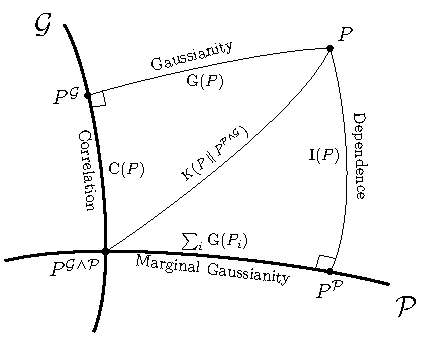
\includegraphics[height = 11cm, width=\textwidth]{../figure_tikz/theory_info}
  \caption{Representation of the distribution and the different projections on the manifolds $\zD P$ and $\zD G$.}
\end{figure}
\end{minipage}
}

As mentioned in~\cite{}, the Pythagorean theorem implies:
\begin{equation}
\label{eqn:pyt}
        \zZ IY + \sum_i\zZ G{Y_i} = \zZ GY + \zZ CY.
\end{equation}
If the mutual information $\zZ I P$ appears to be the best one to use, it is too hard to compute.
The equation \ref{eqn:pyt} justifies the use of the non-gaussianity, correlation or even negentropy as contrast functions.

\end{block}

%% --------- ---- -  -        SEPARATION DE BLOCS         -  - ---- --------- %%

\begin{block}{Performance evaluation}
The ``Amari error'', equation \ref{eqn:amari}, gives a criterion of proximity between two matrices, to evaluate the performance of an algorithm.
If $U$ and $V$ are two $n$-by-$n$ matrices, the Amari error is defined by:
\begin{equation} \label{eqn:amari}
	d(U,V) = \frac{1}{2n}\sum\limits_{i=1}^n \left(\frac{\sum\limits_{j=1}^n|a_{ij}|}{\max_j |a_{ij}|}-1 \right)+\frac{1}{2n}\sum\limits_{j=1}^n \left(\frac{\sum\limits_{i=1}^n|a_{ij}|}{\max_i |a_{ij}|}-1 \right)
\end{equation}
with $a_{ij} = (UV^{-1})_{ij}$.
This function, which is not an actual distance, has the advantage to be invariant by scaling factors and permutation of the components of the matrices.

\end{block}

%% --------- ---- -  -        SEPARATION DE BLOCS         -  - ---- --------- %%

\begin{block}{Algorithms}
Several algorithms have been developed to perform ICA, among those we can cite:
\begin{itemize}
\item HJ: one of the first algorithms for ICA by Hérault and Jutten who pioneered the \textit{blind source separation problem} in the 1980s. It is inspired from the neural network principle.
\item JADE: for Joint Approximate Diagonalization of Eigenmatrices. It belongs to the family of the cumulants algorithms initially introduced by Comon in the early 1990s and has a complexity of $\mathcal{O}(n^4)$.
\item FastICA: proposed by Hyvärinen in the late 1990s, it uses non-gaussianity as an approximation of independence and performs approximate Newton iterations.
\item KernelICA: Introduced in the early 2000s by Bach and Jordan, this method outperforms most of the previous algorithms and is particularly resistant to outliers. However, it is more computationally expensive.
\end{itemize}

\end{block}

%% --------- ---- -  -        SEPARATION DE BLOCS         -  - ---- --------- %%
\begin{block}{Hérault and Jutten (HJ) algorithm}
This method is based on the neural network principle. Writing $W = \zp{I_n+\widetilde W}^{-1}$, for a pair of given functions $\zp{f,\:g}$, the algorithm estimates:
\begin{equation}
\widetilde W_{ij} = f(y_i) g(y_j).
\end{equation}
\end{block}

\end{column}

% Deuxième colonne
\begin{column}{.48\linewidth}



%% --------- ---- -  -        SEPARATION DE BLOCS         -  - ---- --------- %%

\begin{block}{JADE algorithm}
Several methods are based on the cumulants. The aim in JADE is to annul all the cross cumulants of order $4$.
The cumulant tensor is diagonalized which is equivalent to minimizing the following contrast function:
\begin{equation}
  c\zp{x} = \sum_{i,k,l}\zp[b]{\zop{Cum}{x_i,x_i^*,x_k,x_l}}^2.
\end{equation}
\end{block}

%% --------- ---- -  -        SEPARATION DE BLOCS         -  - ---- --------- %%

\begin{block}{FastICA algorithm}
The FastICA algorithm is based on the information theory. Non-gaussianity is used a proxy for independence. Given a quadratic function $f$, the algorithm performs:
\begin{equation}
  \widetilde W_{t+1} = \zesp{X.\ztr{f(\ztr{W_t}X)}} - \zesp{f''(\ztr{W_t}X)}W_t,
\end{equation}
where $W_t$ is the normalized vector of $\widetilde W_t$. For experimentation, we use $f(x) = \frac{x^4}4$.
\end{block}

%% --------- ---- -  -        SEPARATION DE BLOCS         -  - ---- --------- %%

\begin{block}{KernelICA algorithm}
Given a reproducing kernel Hilbert space $\mathcal{F}$, this algorithm seeks to minimize the Kernel Generalized Variance defined as:
\begin{equation}
	\widehat{\delta}_{\mathcal{F}}=-\frac{1}{2}\log \underset{i}{\prod}(1-\rho_i^2)
\end{equation}
where the $\rho_i$ are the kernel canonical correlations between the observations components, obtained with computations over the observations Gram matrices.
\end{block}

%% --------- ---- -  -        SEPARATION DE BLOCS         -  - ---- --------- %%

%\begin{block}{Modus operandi}
%We have consider $m$ distribution of probability, each sampled $N$ times.
%
%We mixed them with a random matrix, whitened this data and apply the ICA algorithm.
%
%Eventually, we compare the matrix found with the true matrix using the Amari error.
%\end{block}

%% --------- ---- -  -        SEPARATION DE BLOCS         -  - ---- --------- %%

\begin{block}{Results}

\begin{figure}
\label{distres}
\centering
\resizebox{\textwidth}{!}{
\input{Tableau_Nathan.txt}
\input{Tableau2.txt}}
\caption{\textbf{Left:} Average Amari error re-scaled by 100 obtained with the listed algorithms for random mix $m=2$ sources of size $N=250$ sampled with twelve different distributions. \textbf{Right:} Same measure for $m$ sources of size $N$ whose distribution is randomly selected among the twelve. The best results are in bold font. An X is put when a standard desktop computer could not compute the result.}
\end{figure}

\begin{figure}
\label{imres}
\centering
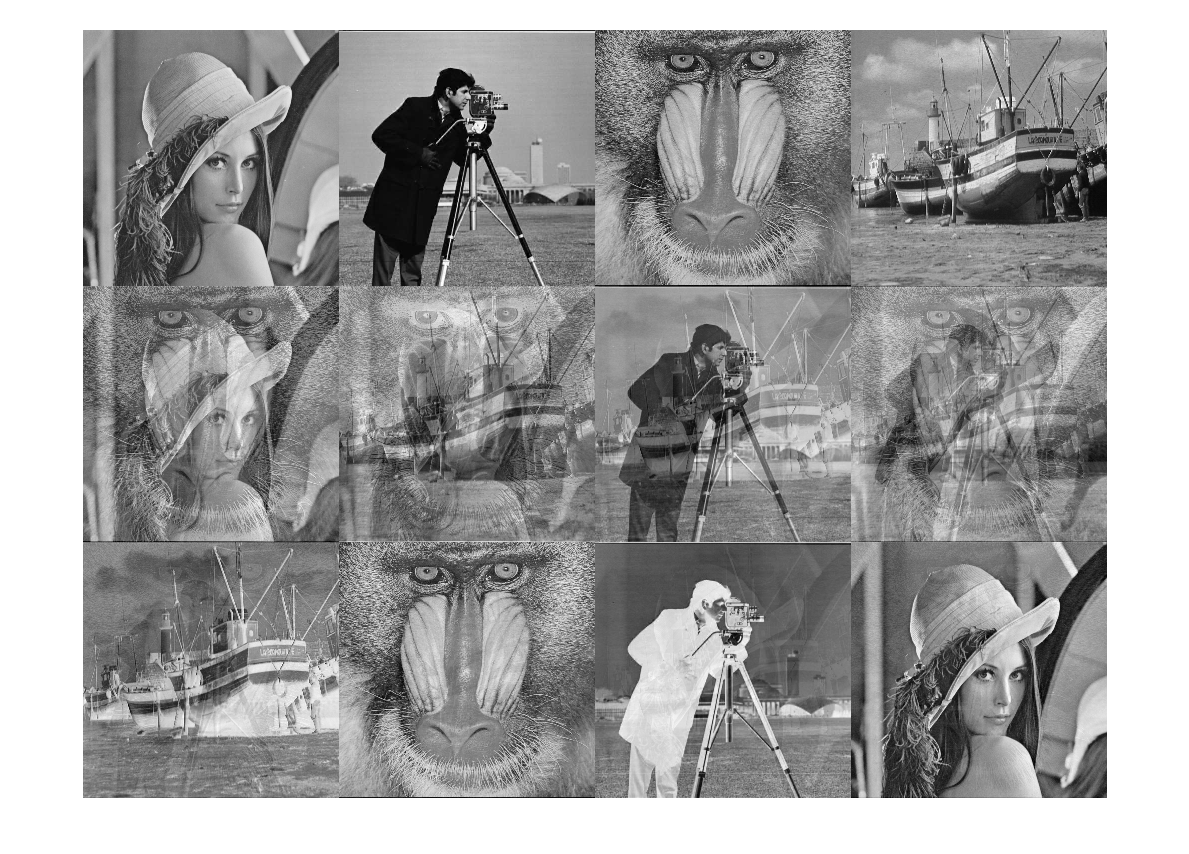
\includegraphics[width=16cm]{../../image_test/unmix4.png}
\caption{Application of JADE algorithm to images separation. The first line presents the original sources, the second one the mix and the last one the estimations.}
\end{figure}
\end{block}

\begin{block}{References}
	\begin{tiny}
\bibliographystyle{alpha}
\bibliography{Biblio}{}
\nocite{*}
	\end{tiny}
\end{block}

\end{column}
\end{columns}

\end{frame}
\end{document}
